\chapter{Introduction}
\label{chapterlabel1}
% Inline citation: \bibentry{example-citation}

\section{Aim}
The aim of this project is to understand how to implement neural network architectures and how they can be implemented given the software available today. The original goal was to create a machine vision tool for understanding emotion but in order to create such a tool one most first understand the basics of machine learning for image and video classification. The project is an exploratory one that follows my initial journey in understanding and implementing neural network architectures for video classification by first recreating architecture for action recognition in videos as presented in \bibentry{KarpathyCVPR14} using TensorFlow and the Keras API.

\section{Theory}
%needs more references%
\subsection{Neural networks}
To first begin we must understand what a neural network is, a neural network is a network of artificial neurons sometimes called a perceptron, a perceptron takes in an inputs $x_i$, and uses trainable weights $w_i$, a bias $b$ and a given activation function to predict the expected output $y_i$. Figure \ref{fig:neuron} provides an image representing a neuron. The activation functions commonly used include 

\begin{equation}
g(z) = \frac{1}{1+ exp(-z)}
 \qquad \text{Sigmoid function}
\end{equation}

\begin{equation}
g(z) = max(0,a)
 \qquad \text{Rectified Linear Unit(RELU) function}
\end{equation}

\begin{equation}
g(z) = \frac{exp(z)-exp(-z)}{exp(z) + exp(-z)}
 \qquad \text{Hyperbolic tangent function}
\end{equation}

\begin{figure}
  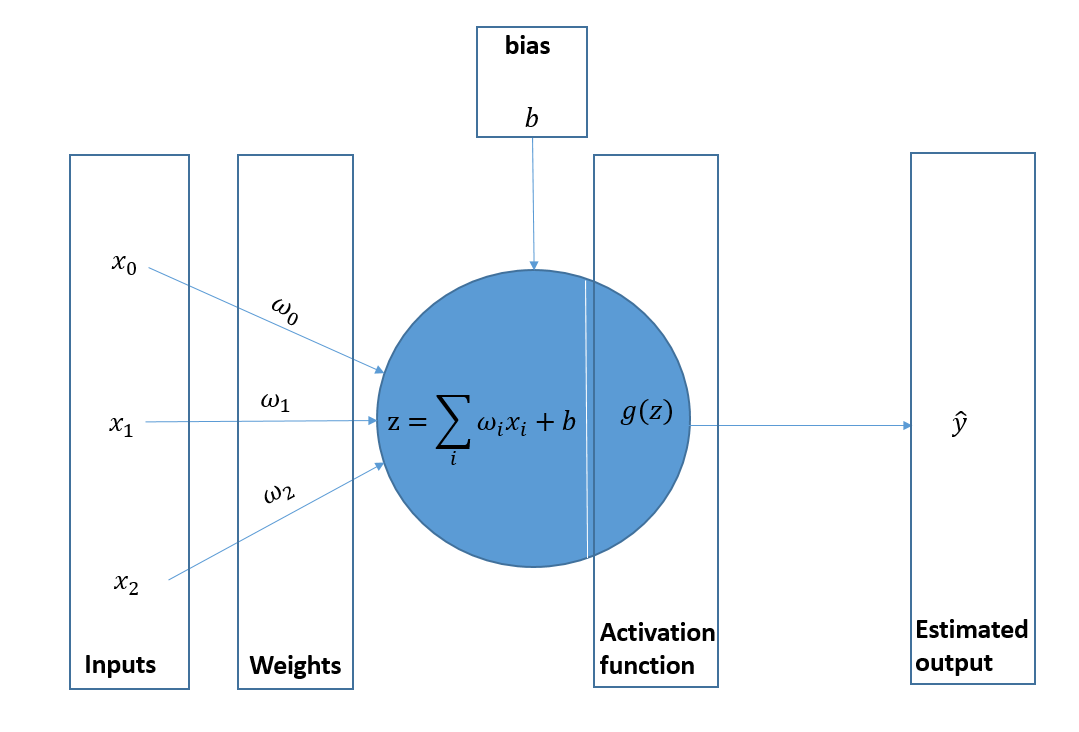
\includegraphics[width=\linewidth, scale=0.2]{neuron.PNG}
  \caption{Neural Network structure}
  \label{fig:neuron}
\end{figure}

To get accurate estimation of the output we have to decide on the weights and bias that would achieve this. One popular algorithm used for this is gradient decent. The gradient decent algorithm works as seen below. 
\begin{enumerate}
 \item  We begin by randomly initialize the weights and the bias
  \item then by what is called Forward propagation compute $z$ as seen in figure \ref{fig:neuron} then expected output given by the activation function. The formular $z$ can also be wriiten as $WX +b$ where  $W$ and $X$ are the matrix representation of the input and weights.
  \item Using a loss function, $\mathcal{L}(\hat{y},y)$ that compares the expected output and the estimated output, we can calculate the loss
  \item Our aim is to minimize this loss as much as possible so we do this by first calculating the partial derivative of the loss function with respect to the weight, $\frac{\partial \mathcal{L}(\hat{y},y)}{\partial W}$ and the bias, $\frac{\partial \mathcal{L}(\hat{y},y)}{\partial b}$
    \item Then using we can update the weight and bias using the below, where $\alpha$ is the learning rate.
\[W = W - \alpha \frac{\partial \mathcal{L}(\hat{y},y)}{\partial W}\]
\[b = b - \alpha \frac{\partial \mathcal{L}(\hat{y},y)}{\partial b}\]
\item We can then repeat step 2 to 5 till difference of current values and the updated values are at a expected threshold.
\end{enumerate}

We can stack these neurons together to from a neural network as seen in Figure \ref{fig:neuralnetwork}, which shows a 2 layer networks with one hidden layer with three neurons. The output of the activation function of the hidden layer servers as an input to the output layer. Usually the more complex the problem the deeper the network.
% maybe find  a diagram of the functions
In terms of activation functions, the RELU function is usually the activation function of choice for hidden layers. This is because there is less of an effect of the slope of the function as it goes to zero which allows for faster learning. The sigmoid function on the other hand is usually used in the output layer for binary classification.

\begin{figure}
  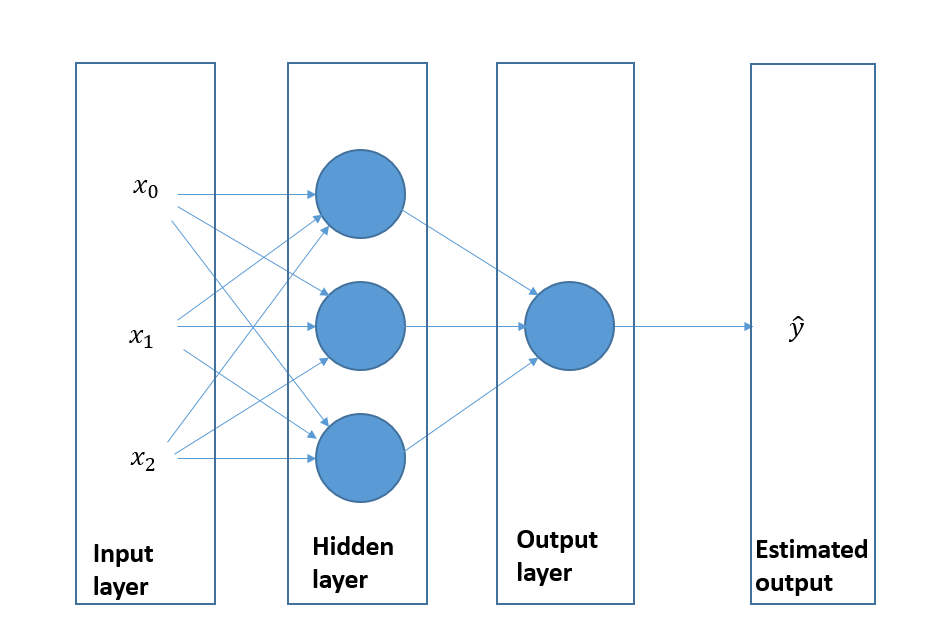
\includegraphics[width=\linewidth, scale=0.2]{multi-layer-network.PNG}
  \caption{Neural Network structure}
  \label{fig:neuralnetwork}
\end{figure}

\subsection{Convolutional Neural networks}
% also explain stride and give the formula for the parameters and where the features come in
Convolutional neural network, which will be the main network of focus in this project is simply a neural network mainly for inputs with a grid structure such as time series data and particularly images. These networks uses a convolution operation in place of a matrix multiple in atleast one of its layers as defined in \citep{Goodfellow-et-al-2016}. The convolution operation is typically represented with an asterisk:s  and seen below representing. 
\[ s(t) = (x * w)(t) \] 
which can be represented as the below, where $x$ is the input and $w$ is the kernal and the output is usually refered to as the feature map.
\[ s(t) = \int x(a) w(t - a)da \] 
In terms for matrices can be written as the below where $I$ for example is a two dimensional image and $K$ is the two dimensional kernel
\[S(i, j) = (I*K)(i, j) = \sum_m \sum_nI(m, n)K(i- m, j- n). \]
Convolutional networks also include a pooling layer which is a applys a function that replaces an input a with a summary statistic of the nearby input.

% \subsection{Optimization}



\section{Context}
    In past few years, with the increase in large labelled datasets such as the Imagenet dataset as discussed in \citep{JiaDeng2009IAlh}, which is an image dataset organized according to the WordNet hierarchy. In this hierachy, a wordnet is a meaningful concept which could also be described by multiple words or word phrases which are called a "synset". In the Imagnet dataset, WordNet contains more than 100,000 synsets, where nouns are the majority of about 80,000 plus. ImageNet aims to provide an average of 1000 images per each synset with the goal of offering tens of millions of images per WordNet. For video data of recent exist the YouTube-8M dataste as dicusssed in \citep{45619}, which a largest multi-label video classification dataset, composed of about 8 million videos for Youtube annotated with a vocabulary of 4803 visual entities. One intresting fact about the Youtube-SM dataset is that a Deep CNN pre-trained on ImageNet was also used to extract the hidden representation immediately prior to the classification layer showing how the available of large datassets can lead to progress in others. Not only have these datasets lead to growth with other datasets but most importantly they have also lead to a rise of various machine learning algorithms used to solve a diverse set of problems. Not only has the increase in datasets helped with this growth but also the increase in the available frames works and libraries used to create these various algorithms. some of these frameworks and libraries used for machine learning include scikitlearn which is a python programming language based library with a long range of user friendly API's for creating machine learning algorithms. \citep{DBLPjournalscorrBuitinckLBPMGNPGGLVJHV13} details the use of scikitlearn and its elegant APIs which has lead to a growth in implementation of models in the machine learning space. In the deep learning space, surveys such as \citep{Nguyen2019} have been taken on the available libraries and frameworks for deep learning with large datasets and the hardware requirements some of these frames works propose.\citep{Wang2019}, is another survey that details the more commonly used deep learning frame works developed by large software houses such as Google, Facebook, and Microsoft, and those developed by the open source community such as Caffe, Caffe2, Tensorflow, MXNet, CNTK, Torch, PyTorch,  MatconvNet, Matlab deep learning and Deep learning tool box, Deeplearning4j to name a few.
    For the purpose of this paper we will be looking at using Tensorflow and keras libraries and APIs with python as the programming language for building and using popular models. 
    Where Tensorflow is a free and open-source software library developed by Google and released in November 2015 for dataflow and differentiable programming as described in \citep{8578572} and keras as discussed in \citep{Lux:2019:OSC:3310195.3310202} is a high-level elegant neural networks API that provides tools for easy constructions of models. It also provides access to popular pre-trained models and it is capable of running on top of frameworks like TensorFlow, CNTK, or Theano. 
    This paper will be looking to experiment with how to implement neural network architectures for video classification particularly looking into deep convolutional neural networks which have been applied to a large pool of visual tasks since the late 1980s as discussed in \citep{doi:10.1162neco_a_00990}.
        % maybe add here more on video classification and temporal issues
    % Although primary used for image classification this paper will also be looking at the
    
        \section{Related Work}

% talk abour related work here on other models for video classification double check the pedistrain dection paper% 
There is vast range of problems in which convolutional neural network(CNNs) architectures are used, some of which are in the image classification space which include problems such as object detection for example in pedestrian detection \citep{TomeD2016DCNN} systems, to speech  recognition problems and also facial and body recognition systems which are items in the human emotion recognition and human interaction space \cite{knyazev2017convolutional} .They have also been used in natural language processing for example with modelling sentences as explained in \cite{Kalchbrenner_2014}. 
Most importantly, CNNs have also been used for video classification for example by using the codec as a spatio-temporal Activity Sensor on videos as described in \citep{ChadhaA2017VCWC}. Apart from convolutional neural networks there are other machine learning methods used for example bag of words models \citep{10.1007978-3-642-28493-9_34}, this can be based on using local visual descriptors, most common of these are histogram of oriented gradients (HOG), histogram of optical flow (HOF) and motion boundary histograms (MBH) descriptors which are very powerful for classification but also computationally expensive as described in \citep{Uijlings2015}. Other methods use recurrent neural networks(RNNs) which is also used in the natural language processing space and in general for sequence data. Since videos are essentially sequence data, RNNs can be used in theory however because RNNs are difficult to train on high-dimensional inputs due to the large input-to-hidden weight matrix there has been some difficulty using them, however there is additional research in the space that has lead to competitive results such as that described in \citep{yang2017tensortrain} which factorizes the input-to-hidden weight matrix using Tensor-Train decomposition to help with efficiency of training these models.
% reference need for von Neumann bottleneck and https://cloud.google.com/blog/products/ai-machine-learning/what-makes-tpus-fine-tuned-for-deep-learning%
Also when running these models apart from architecture one has to also consider processing hardware as evaluated in \citep{wang2019benchmarking} as this has an effect performance. Devices range (Central processing units) CPUs, which reads each instruction from the software hence has to store all calculaculations internally on memory. This memory access becomes the downside of CPU architecture called the von Neumann bottleneck because each CPU's Arithmetic Logic Units (ALU) executes calculation one by one, accessing the memory every time, limiting the total throughput and consuming significant energy. Another is the GPU(Graphical processing units which uses thousands of ALUs(about 2,500–5,000) in a processor of ALUs which means it can then execute thousands of multiplications and additions simultaneously. However it still suffers from the von Neumann bottleneck because For every  calculation in the thousands of ALUs, GPU it still needs to access shared memory to read and store intermediate calculation results. The most recent device of late is the Google designed, TPU (Tensor Processing Unit), which is designed as a matrix processor specialized for neural network work loads and is not as affected by the von Neumann bottleneck because its' primary task is matrix processing hence it consist of thousands of multipliers and adders connected to each other directly to form a large physical matrix called the systolic array architecture. Hence calculations naturally flow through the architecture reducing memory access during calculation and as a result it has a high computational throughput on neural network calculations with much less power consumption and smaller footprint.
%   todo add how easy it is to implement to bring it all together
  
%   such as there is a range of models typically used such as -----, videos can also be looked and complication of images in frames which simple convolutional networks can be use to classify together with methods used to take into account the temporal features. 
  
%   talk about vido clasification
    % This models have produced great results when it comes to image classification as discussed further in papers such as \citep{MISHKIN201711}. The use of convolutional neural networks doesn't stop in the computer vision field with image classification and video classification but also extends to tas well as physiological data, speech to name a few.
    
% why tensor flow this is a good paper \citep{schrimpf2016i}

    % When looking to build most reasches beging by either devloping there own neural network and looking at the archetures of other. one of the issue faces is the the same computational pwoer and hypter paraametres found.


